\begin{englishtitle}
\title{Application of graph theory to modeling\\
the semantic text structure}
% First author
\author{M.~A.~Skurygina\inst{1},
P.~Yu.~Solodusha\inst{2}}
\institute{Institute of Mathematics and Information Technologies\\Irkutsk State University, Irkutsk, Russia\\
  \email{skurygina-maria@yandex.ru}
  \and
Institute of Philology, Foreign Languages, and Media Communication\\Irkutsk State University, Irkutsk, Russia\\
\email{peter.solodusha@mail.ru}}
% etc

\maketitle

\begin{abstract}
The report addresses an approach to constructing models in mathematical linguistics based on the stochastic graphs tool. We present the results obtained from the analysis of the semantic scheme of the in-depth interview.

\keywords{graph theory, mathematical modeling, mathematical linguistics}
\end{abstract}
\end{englishtitle}

\iffalse
\documentclass[12pt]{llncs}
\usepackage[T2A]{fontenc}
\usepackage[utf8]{inputenc}
\usepackage[english,russian]{babel}
\usepackage[russian]{nla}

\usepackage{xcolor}

%\usepackage[english,russian]{nla}

% \graphicspath{{pics/}} %Set the subfolder with figures (png, pdf).

%\usepackage{showframe}
\begin{document}
%\selectlanguage{russian}
\fi

\title{Применение теории графов для моделирования семантической структуры текста%\thanks{Работа выполнена при поддержке РФФИ (РНФ, другие фонды), проект \textnumero~00-00-00000.}
}
% Первый автор
\author{М.~А.~Скурыгина\inst{1}
\and
% Второй автор
П.~Ю.~Солодуша\inst{2}}

\institute{Институт математики и информационных технологий\\ Иркутский государственный университет, Иркутск, Россия\\
  \email{skurygina-maria@yandex.ru}
  \and
  Институт филологии, иностранных языков и медиакоммуникации\\ Иркутский государственный университет, Иркутск, Россия\\
  \email{peter.solodusha@mail.ru}
  }



\maketitle

\begin{abstract}
В докладе рассматривается подход к построению моделей в математической лингвистике на основе аппарата стохастических графов. Приведены результаты, полученные при анализе семантической схемы глубинного интервью.



\keywords{графы, математическое моделирование, математическая лингвистика}
\end{abstract}

 
На современном этапе развития математической лингвистики 
при разработке языковых концепций используется понятийный аппарат из теории множеств [1], теории игр (J.~Hintikka, L.~Henkin), теории нелинейных динамических систем [5]. Для анализа структуры текста исследователи привлекают теорию вероятностей и оптимизацию (дистрибутивную семантику), а также теорию графов [3,~4].

В докладе рассматривается применение теории стохастических графов для построения семантической модели текста (см., например, [3]). Для реализации была выбрана семантическая схема из [4, с.~115]. Она содержит шесть наиболее часто встречающихся микротем в тексте глубинного интервью [2] и проиллюстрирована в виде  ориентированного графа, приведенного на рис. 1. Его вершины -- микротемы (1 -- <<Я>>, 2 -- <<Действие>>, 3 -- <<Место>>, 4 -- <<Количество>>, 5 -- <<Семья>>, 6 -- <<Человек>>), а рёбра -- переход от одной микротемы к другой.
 


\begin{figure}
    \begin{center}
        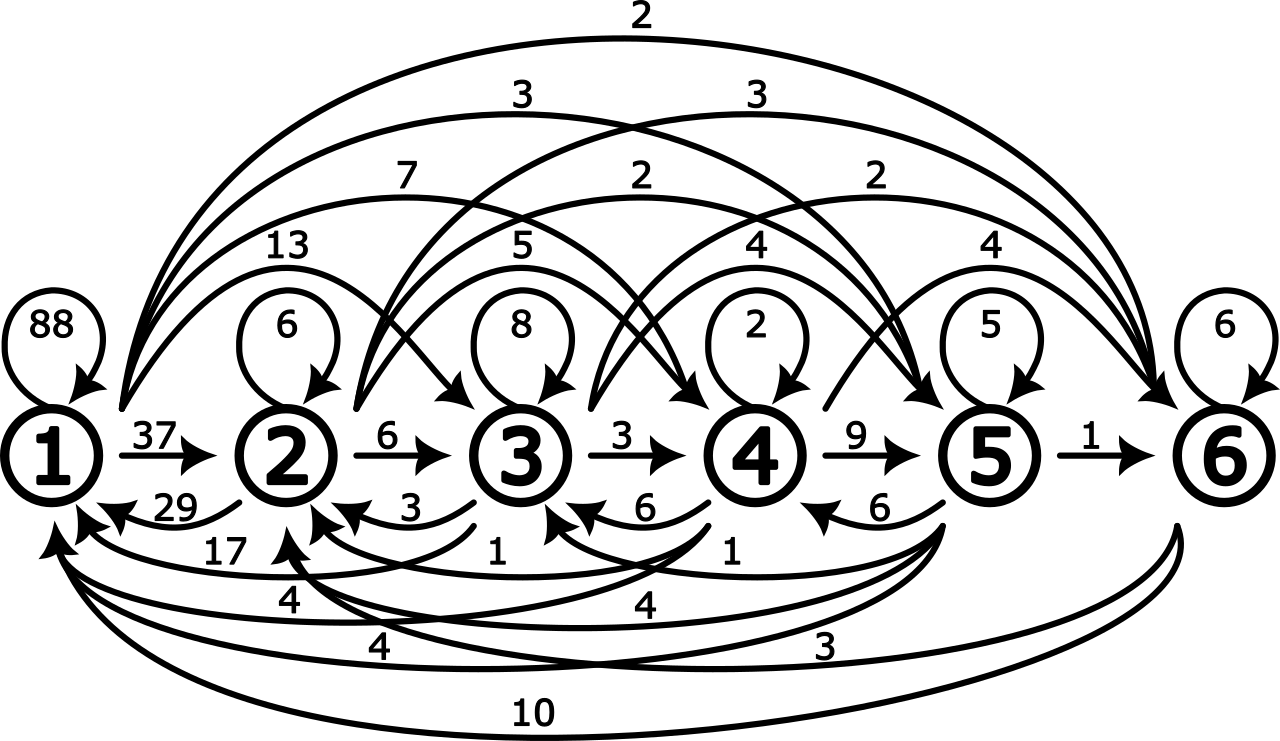
\includegraphics[height=5cm]{skurygina_solodusha.png}
    \end{center}
    \caption{Граф, соответствующий изучаемой семантической схеме}
    \label{fig1}
\end{figure}



Анализ показал, что данный граф является взвешенным, т. е. все вершины и рёбра имеют вес. Вес вершины определяется количеством слов из выбранных микротем, а вес ребра соответствует числу переходов между микротемами. Вершины графа упорядочены по убыванию значений веса. В рассматриваемом случае граф является насыщенным. При увеличении выборки микротем до десяти наименований (дополнительно внесены: <<Эмоциональное состояние>>, <<Движение>>, <<Возраст>>, <<Отождествление>>) граф становится разреженным по терминологии [3]. Основные результаты связаны с исследованием свойств данного графа, зависящих от размера выборки. 


% Список литературы.
\begin{thebibliography}{99}

% Format for Journal Reference:
% Author1 N., Author2 N.  Article title. Journal. Year. Vol.~Volume, No~Number. Pp.~Page numbers.
% Format for books:
% Author N. Book title. Place: Publisher, year.
% Format for Russian Journal Reference:
% Фамилия И.О. Название статьи~// Журнал. Год. Т.~том,  \textnumero~номер. С.~страницы.
\bibitem{1}
Баевский~В.~С. Лингвистические, математические, семиотические и компьютерные модели в истории и теории литературы. М.: Языки славянской культуры, 2001.
\bibitem{2}
Михалёва~О.~Л., Васильева~Е.~В., Стародворская~Е.~В., Ташлыкова~М.~Б. Глубинное интервью как материал для лингвистического исследования. Иркутск: Изд-во ИГУ, 2013. С.~19--38.
\bibitem{3}
Райгородский~А.~М. Модели интернета. Долгопрудный: Издательский Дом <<Интеллект>>, 2013.
\bibitem{4}
Рачёва~А.~А., Стребкова~К.~Е. Что скрывается в глубинах человеческого <<я>>, или анализ одной графосемантической модели ментальной репрезентации <<значимого другого>>~// Студенческие психологические чтения: от науки к практике. 2021. С.~110--119.
\bibitem{5}
Трубецков~Д.~И., Трубецкова~Е.~Г. Фрактальное искусство~// Известия вузов. Прикладная нелинейная динамика. 2016. \textnumero~6. С.~84--103.
% etc
\end{thebibliography}


% Обязательная информация на английском языке:




%\end{document}
